\chapter{Literature Review}
 
%%%%%%%%%%%%%%%%%%%%%%%%%%%%%%%%%%%%%%%%%%%%%%%%%%%%%%%%%%%%
%%%%%%%%%%%%%%%%%%%%  NEW SECTION   %%%%%%%%%%%%%%%%%%%%%%%%
%%%%%%%%%%%%%%%%%%%%%%%%%%%%%%%%%%%%%%%%%%%%%%%%%%%%%%%%%%%%
\setcounter{equation}{0}

\section{System Description}

The system can be described based on the five phases: 
   \begin{enumerate}
        \item  Utilizes Large Language Models (LLMs) to interpret and process natural language user queries. 
        \item Translates interpreted queries into actionable instructions and generates JSON files. 
        \item Executes transactions based on JSON instructions by interacting with financial systems.
	\item Manages the secure storage and retrieval of transaction data using a connected storage bucket.
        \item Enforces user permission protocols to control access and ensure data protection.
    \end{enumerate}

\noindent The system developed in this project is structured around several key components: the Natural Language Processing (NLP) Interface, which utilizes Large Language Models (LLMs) to interpret and process user queries in natural language; the Processing Engine, which translates these interpreted queries into actionable instructions and generates corresponding JSON files; the Action Model, which executes the specified transactions by interacting with underlying financial systems; Data Management, which involves the secure storage and retrieval of transaction data using a connected storage bucket; and Security Protocols, which enforce robust user permission controls to manage access and ensure data protection. This integrated approach ensures a user-friendly, efficient, and secure transaction processing system that meets the evolving needs of modern financial systems. 

\begin{figure}[h!]
    \centering
    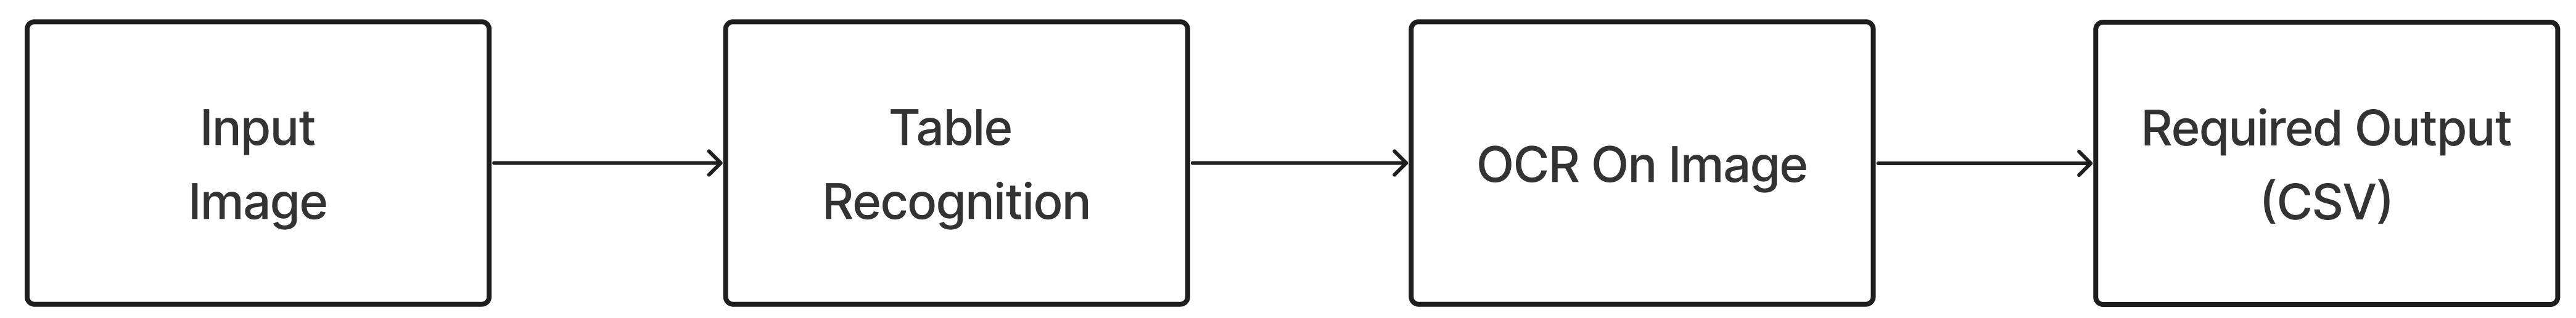
\includegraphics[width=1\textwidth]{Images/lit_review/Initial concept of our system.jpg}
    \caption{Initial concept of the system}
\end{figure}

\clearpage

\section{Existing Solutions}

\noindent
The system description was based on the initial concept that was pitched before extensive research. The phases of this system concept may have existing solutions of various implications and importance which will be explored below.\\

\noindent
J. Smith et al. [1] proposed {\it Mistrell 7b: Advancements in Artificial Intelligence} in 2024.
\noindent
This paper focuses on using advanced language models to process and understand complex user queries in natural language, facilitating more intuitive interaction with financial systems. Mistrell 7b demonstrates significant improvements in language comprehension and transaction accuracy. \\

\noindent
John Doe et al. [2] proposed {\it LLaMA: Open and Efficient Foundation} in 2023. 
\noindent
This paper discusses the development of the LLaMA (Large Language Model Architecture) framework, which aims to create an open and efficient foundation for natural language processing tasks. The authors highlight the system's design principles, which focus on optimizing computational efficiency and accessibility. LLaMA is designed to handle a wide range of language processing tasks with high accuracy and speed, making it suitable for various applications, including transaction processing.\\

\noindent
L. Zhang [17] proposed {\it Improvement of Voice Navigation System based on Customer Service} in 2023. 
\noindent
The paper focuses on enhancing voice navigation systems through a customer service-oriented approach. By leveraging advancements in artificial intelligence and natural language processing, Zhang proposes improvements to voice-based navigation systems to better cater to customer needs and preferences. The paper discusses techniques for enhancing voice recognition accuracy, optimizing user interactions, and improving overall user satisfaction with voice navigation systems.\\

\noindent The above discussed literature provides advanced capabilities that  can significantly enhance various aspects of transaction processing systems, from improving user interaction and automation to ensuring accuracy and efficiency in handling financial data. \\

\noindent
J. Wu et al. [12] proposed {\it TidyBot: Personalized Robot Assistance with Large Language Models} in 2023.
\noindent
This paper introduces TidyBot, a personalized robot assistant powered by Large Language Models (LLMs). TidyBot utilizes advanced natural language processing techniques to understand and respond to user commands, providing personalized assistance in various tasks. The system leverages the capabilities of LLMs to interpret natural language inputs and generate contextually relevant responses.\\

\noindent
S. Zou et al. [13] proposed {\it Large Language Models in Healthcare: A Review} in 2023. 
\noindent
The paper provides a comprehensive review of the application of Large Language Models (LLMs) in the healthcare domain. The authors explore how LLMs, such as GPT-3 and BERT, are being utilized to address various challenges in healthcare, including medical diagnosis, electronic health record (EHR) management, patient communication, and medical research. The review discusses the capabilities of LLMs in understanding and generating medical text, their potential impact on clinical decision-making, and the challenges associated with their implementation in healthcare settings.\\

\noindent
The above two references contribute to the understanding and utilization of LLMs in different contexts, providing valuable insights for tasks involving language processing, understanding, and generation.\\

\noindent
A. L. Sinha et al.[4] proposed {\it AI based Desktop Voice Assistant for Visually Impaired Persons} in 2023.
\noindent
The paper introduces an innovative desktop voice assistant system designed specifically to aid visually impaired individuals in performing various tasks. By leveraging artificial intelligence (AI) technology, particularly natural language processing (NLP) techniques, the system interprets voice commands and executes corresponding actions, providing a seamless user experience for individuals with visual impairments.\\

\noindent
M. Bombothu et al.[18] proposed {\it INTELLINEO – An Intelligent Personal Assistant} in 2023.
\noindent
The paper introduces INTELLINEO, a personal assistant that utilizes advanced artificial intelligence techniques, including natural language processing and machine learning, to understand user queries and provide contextually relevant responses. The system aims to enhance user productivity and efficiency by automating routine tasks, such as scheduling appointments, managing emails, and accessing information from databases. \\

\noindent
K. N. Lam et al. [14] proposed {\it A Transformer-Based Educational Virtual Assistant Using Diacriticized Latin Script} in 2023. 
\noindent
The paper aims to enhance educational experiences by providing personalized assistance to users in learning activities. By leveraging transformer-based architectures, such as BERT or GPT, the virtual assistant can understand and respond to user queries with high accuracy. Additionally, the integration of diacriticized Latin script enhances the system's ability to handle diverse linguistic inputs, catering to a wider range of users with varying language preferences.  \\

\noindent
S. P. Yadav et al. [9] proposed {\it Voice-Based Virtual-Controlled Intelligent Personal Assistants} in 2023.
\noindent
The paper focuses on leveraging voice commands for controlling intelligent personal assistants in financial transactions. The system utilizes advanced natural language processing techniques to interpret voice commands, allowing users to interact with financial systems in a more intuitive and accessible manner. \\

\noindent
These research papers can be used to gather insights and ideas for the development of various tasks related to intelligent personal assistants and virtual assistants. 

\clearpage



\section{Summary}

\noindent 
The literature review presented a thorough examination of different research studies and works relevant to the proposed system. It offered valuable insights and multiple potential solutions for addressing each phase of the development of the system.

\vspace{3mm}

\noindent
The project aims to develop an innovative transaction processing system leveraging Large Language Models (LLMs) to enhance user interaction and system efficiency. Drawing inspiration from recent advancements in LLM technology and their applications across various domains, including healthcare, education, robotics, and personal assistance, the project seeks to harness the power of natural language processing to revolutionize transaction processing methodologies.

\vspace{3mm}

\noindent
Building upon existing research, such as {\it"The Recent Large Language Models in NLP"} and {\it"TidyBot: Personalized Robot Assistance with Large Language Models"} the project adopts a comprehensive approach to integrate LLMs into a transaction processing framework. By analyzing the capabilities and potential applications of LLMs in different contexts, the project aims to develop a system that enables users to perform transaction-related tasks effortlessly using natural language commands.

\noindent
Furthermore, insights from papers like {\it"Voice-Based Virtual-Controlled Intelligent Personal Assistants"} and {\it"AI-based Desktop Voice Assistant for Visually Impaired Persons"} inform the project's design considerations, emphasizing the importance of user-friendly interfaces and accessibility features. By incorporating voice-based interaction and assistive technologies, the system aims to cater to diverse user needs, including those with visual impairments.

\vspace{3mm}

\noindent
Additionally, the project draws upon research on LLMs in healthcare, education, and customer service automation to enhance the security, efficiency, and personalized assistance features of the transaction processing system. Papers such as {\it"Large Language Models in Healthcare: A Review"} and {\it"A Transformer-Based Educational Virtual Assistant Using Diacriticized Latin Script"} provide valuable insights into the potential benefits and challenges of integrating LLMs into real-world applications.

\vspace{3mm}

\noindent
In summary, the project seeks to leverage the advancements in LLM technology and insights from relevant literature to develop a transaction processing system that offers intuitive user interaction, accessibility, security, and personalized assistance. By combining state-of-the-art natural language processing techniques with domain-specific knowledge, the project aims to contribute to the evolution of transaction processing methodologies, catering to the needs of modern users in an increasingly digital world.

\vspace{3mm}

\noindent
According to this, each phase of the proposed system is planned, which will be discussed in the subsequent chapter.

